% !TEX root = manualLatexMavenPlugin.tex

\chapter{Graphical Preprocessing}\label{chap:GraphConversions}

While \LaTeX{} is really strong in text processing 
and also in formula processing, 
in itself it is weak in its graphical abilities. 
Graphics in some formats can be included directly, 
in some cases preprocessing is necessary to obtain includable graphics, 
but in most cases, according \LaTeX-packages must be used: 
%
\begin{itemize}
\item[graphicx]
is the basic graphics package which provides the command 
\cmd{includegraphics}{} 
which allows including graphics natively 
in the formats pdf, eps, jpg and png at least. 
For details see~\cite{GraX}. 
\item[xcolor]
allows using colors in graphics. 
Even if the author does not use colors in graphics, 
several formats, like \gls{fig}, \gls{gp} and \gls{svg} 
offer it and so the according converters 
transforming them into the native formats 
create color information which can be rendered only via \texttt{xcolor}. 
For details see~\cite{XColorP}. 
\item[transparent]
allows specifying transparency in graphics. 
Here the same applies as for color: 
Even if you do not use the feature, 
some source formats do (in fact only \gls{svg}) does 
and so the according converters create according information 
and so \LaTeX{} must get along with it. 
For details see~\cite{TransP}. 
\item[bmpsize]
is needed for bitmap formats like \gls{jpg} and \gls{png} only. 
Used to extract resolution and bounding box. 
FIXME\@: needed more information. 
For details see~\cite{BmpP}. 
\item[tikz]
The tikz code described in \cite{TikzPGF} is just in \LaTeX{} format. 
Thus, it can be included directly anddoes not require any preprocessing. 
Still what is needed is a good graphical editor like \texttt{tikzedt} 
with online manual \cite{TikzEdt}. 
\item[import]
is strictly speaking no graphics package. 
According to its documentation~\cite{ImpoP}, 
it allows an imported file to find its own inputs 
(using ``\cmd{input}'', ``\cmd{includegraphics}'' etc.) in that directory. 
This is vital for the graphic formats for which a tex-file is imported 
which itself imports a pdf/eps file located in the same folder 
but not in the folder of the importing file. 
It is advisable to combine the \texttt{import} package with other graphic packages 
to include graphics in separate graphic files. 
\item[pythontex]
is strictly speaking no graphics package either but more general 
a way to include and run code within a \LaTeX{} document 
as described in~\cite{PythonTexP}. 
Note that not only Python but also other languages can be used. 
Most of them offer graphic capabilities 
and so graphics can be included also via \pkg{pythontex}. 
Nevertheless, we do not treat this technique in this chapter, 
but separately in Section~\ref{sec:pythontex}. 
This is because graphics is a side aspect of \pkg{pythontex} 
and also because strictly speaking there is no preprocessing. 
First a latex processor is run and the package extracts the code 
into a separate file which is then further processed by an external tool. 
This is more like running \cmd{bibtex} to extract a bibliography. 

If using the package \texttt{pythontex} 
a special processing interacting with the latex to pdf converter is required also, 
but it is not preprocessing. 
\end{itemize}

We support figures created in the \gls{fig} by the program xfig, 
figures created by the plotting utility \texttt{gnuplot}, 
the tex-specific graphic language metapost, 
figures in \gls{svg}-format 
and finally figures in formats which can be included into a \LaTeX-file 
without preprocessing like \gls{png} and \gls{jpg}. 
Further functionality on \LaTeX{} figures can be easily added. 
If there is some need, please write an email to the author. 

Table~\ref{tab:graphicOverview} gives an overview over the supported formats 
together with the graphic converters, 
the name of the parameter to configure which one is used 
and the default value. 
Of course this converter must be installed. 
It is advisable to have also an editor installed. 
Sometimes the editor is used also as converter. 
For human readable formats like \texttt{fig}, it often makes sense, 
to use both the graphical editor and the textual one. 

\begin{longtable}{|l|ll|}
\toprule
Graphic format & conversion tool & editor \\
\midrule
\midrule
\endfirsthead%
\bottomrule
\caption{\label{tab:graphicOverview} 
Overview over the supported graphic formats }
\endlastfoot%
fig             & \texttt{fig2devCommand}, e.g.~\texttt{fig2dev}  & xfig, emacs   \\
gnuplot (gp)    & \texttt{gnuplotCommand}, e.g.~\texttt{gnuplot}  & emacs         \\
metapost (mp)   & \texttt{metapostCommand}, e.g.~\texttt{mpost}   & emacs         \\
svg             & \texttt{svg2devCommand}, e.g.~\texttt{inkscape} & inkscape      \\
jpg, png        & ---        & gimp          \\
\end{longtable}

Besides the converter external to \LaTeX, 
also several \LaTeX-packages are required 
to use graphics. 


This section describes the conversions of 
graphical source files into target files 
in detail. 

But pdf also occurs as an intermediate format for pictures. 
For historical reasons, still \gls{eps} is used. 
Section~\ref{sec:figpdf} shows that it suffices to stick to pictures 
in pdf-format. 
% FIXME\@: REALLY? 
%FIXME\@: missing pdf als basic input format. What about (e)ps? 
Section~\ref{sec:fig2dev} shows how \texttt{fig2dev} converts fig-files 
into \LaTeX-files containing text and including graphics in as pdf-files. 
Likewise, Section~\ref{sec:gnuplot2dev} describes 
how gnuplot converts gnuplot-files into pdf-files. 
An interesting alternative to gnuplot for computing pictures 
is metapost described in Section~\ref{sec:metapost}. 
A more elaborate alternative to fig-pictures are svg-pictures 
described in Section~\ref{sec:picSvg}
Also several formats collected in Section~\ref{sec:picasis} 
may be included as is. 



\section{Including pdf-files}\label{sec:figpdf}

Modern \LaTeX{} implementations directly create pdf-files. 
Thus it makes sense, to allow including graphics as pdf-files 
in \LaTeX-files. 
This is done in pdf mode 
by the \LaTeX-packages \pkg{xcolor} and \pkg{graphicx}. 
In contrast, traditionally \LaTeX{} produced output in the \gls{dvi}-format 
which is still used to create \gls{html}-output, 
this is not supported by the default driver, 
Instead it shall be used the driver \texttt{dvipdfmx}. 
To obtain a \LaTeX-file which works both for creating pdf and html, 
insert in the header of the \LaTeX{} main file
given by Listing~\ref{lst:header}. 
%
%\lstset{language=tex, basicstyle=\small}
% FIXME\@: nag complains for htlatex 
\lstinputlisting[firstline=20, lastline=22,
language=tex, basicstyle=\small,
float, captionpos=b, label={lst:header}, 
caption={From the header of the tex-source of this manual}]%
{header.tex}

An alternative, which we do not use 
is replacing the pdf by an \gls{eps} via configuration file \texttt{myxhtml.cfg} 
which is given by Listing~\ref{lst:xhtml}. 
%
%\lstset{language=tex, basicstyle=\scriptsize}
% FIXME\@: nag complains for htlatex 
\lstinputlisting[language=tex, basicstyle=\scriptsize,
float, captionpos=b, label={lst:xhtml},
caption={Configuration file \texttt{myxhtml.cfg}}]
{myxhtml.tex}
%
It applies when converting \LaTeX{} into html and that like 
with htlatex if invoking something like \texttt{htlatex xxx.tex myxhtml,\ldots} 
where \texttt{myxhtml} is located in the same directory as the \LaTeX-file 
to be processed. 
The configuration file essentially contains a graphics configuration, 
which applies conversion to pdf-files included in the \LaTeX-file \texttt{xxx.tex}
via \cmd{includegraphics}. 


\section{Conversion of fig-files}\label{sec:fig2dev}

\index{xfig}
\index{fig2dev}
A simple but still useful tool to draw figures is \texttt{xfig} 
which stores graphics in a native format 
described in~\cite{XFigF} with file extension \texttt{.fig}. 
The file extension \texttt{.fig} is also used by matlab to store plots 
but this is something different. 
Graphics in xfig format cannot be directly included in latex files 
but must be exported into a \LaTeX-readable format. 

To export a file \texttt{xxx.fig} residing in directory \texttt{yyy} 
into several external formats, 
\texttt{xfig} uses \texttt{fig2dev}. 
A look in~\cite{XFigF}, Section~3.4 shows that texts with set ``special''-flag 
are interpreted as latex-code. 
For these texts the appropriate export language would be \texttt{latex}. 
On the other hand, \texttt{latex} is weak in graphics 
and \texttt{pdf} would be the ideal export format for all kinds of objects, 
except for texts with set ``special''-flag. 
In \texttt{pdf} format, texts are interpreted literally, 
independent of the ``special''-flag. 
Thus \texttt{fig2dev} offers a mixed solution: 
export \texttt{xxx.fig} in format \texttt{pdftex} which yields a pdf-file 
\texttt{xxx.pdf} containing all but text with set ``special''-flag 
and complementary \texttt{pdftex\_t} which yields a tex-file \texttt{xxx.ptx} 
including the pdf-file and the texts with set ``special''-flag. 
\index{special-flag}%maybe glossary 
The exported files are in the same directory \texttt{yyy} 
as the original file \texttt{xxx.fig}. 

For example, 
the fig-file \texttt{F4\_01fig2dev.fig} defining Figure~\ref{fig:fig2dev}, 
is transformed into a file \texttt{F4\_01fig2dev.ptx} 
in format \texttt{pdftex\_t} which starts as given by Listing~\ref{lst:ptx}. 

%\lstset{language=tex, breaklines, basicstyle=\footnotesize}
% FIXME\@: nag complains for htlatex 
\lstinputlisting[language=tex, basicstyle=\tiny,
breaklines, lastline=25,
float, captionpos=b, label={lst:ptx}, 
caption={The ptx-file for a fig-file}]{F4_01fig2dev.ptx}

The file \texttt{xxx.ptx} is ``imported'' into the tex-file of this manual 
by the command 
%
\begin{lstlisting}[language=TeX]
\import{yyy}{xxx.ptx}
\end{lstlisting}
%texttt
and includes \texttt{xxx.pdf} automatically the file \texttt{xxx.pdf} 
via \cmd{includegraphics\{xxx\}}{} (line 2). 
Note the following remarkable details: 
%
\begin{itemize}
\item
Observe that we can drop the suffix of the included file \texttt{xxx.pdf} 
which is expressed as ``\texttt{xxx}'' 
because \LaTeX{} chooses the right suffix: 
If instead of \texttt{xxx.pdf} there is a file \texttt{xxx.eps}, 
the latter is chosen if no suffix is specified. 
As we will see below, 
omitting the suffix is crucial to make \texttt{xxx.ptx} work 
for both \LaTeX-output formats: 
the pdf-format can include pdf-files, 
whereas the dvi-format which is required to create html- and
odt-files can include eps-files. 
\item
If \texttt{xxx.pdf} is included in \texttt{xxx.ptx} 
with the full path name, 
we may use \cmd{input\{xxx.ptx\}}{} instead of \cmd{import\{yyy\}\{xxx.ptx\}}. 

If in contrast, \texttt{xxx.pdf} is included in \texttt{xxx.ptx} 
with the short name only, 
\texttt{xxx.pdf} is assumed to be in the same directory 
as the file inputting \texttt{xxx.ptx}. 
So in general, i.e.~if this is not \texttt{yyy}, we need import 
\cmd{import\{yyy\}\{xxx.ptx\}}. 
If the directories coincide, 
in the import the string \texttt{yyy} may be empty. 
If the string \texttt{yyy} is not empty, it must end with the path delimiter, 
i.e.~\texttt/ for Unix like systems and 
\texttt{\textbackslash} for win-like systems. 
\end{itemize}

As indicated in Section~\ref{sec:figpdf}, 
the commands in \texttt{xxx.ptx} 
require the packages \pkg{graphicx} and \pkg{xcolor}. 
Also the \cmd{import}{} command 
requires the \pkg{import} package. 

To export \texttt{xxx.fig} into \texttt{xxx.ptx} and \texttt{xxx.pdf} 
this software invokes two commands: 
%
\begin{Verbatim}[fontsize=\scriptsize]
fig2dev -L pdftex   <fig2devGenOptions> <fig2devPdfEpsOptions>        xxx.fig xxx.pdf   
fig2dev -L pdftex_t <fig2devGenOptions> <fig2devPtxOptions>    -p xxx xxx.fig xxx.ptx
\end{Verbatim}
%
Both commands specify the input file \texttt{xxx.fig}, 
both use the options given by the parameter \texttt{fig2devGenOptions} 
while each invocation allows to specify also specific options, 
\texttt{fig2devPdfEpsOptions} and \texttt{fig2devPtxOptions}, respectively, 
and both use the option \texttt{-L} 
to specify the output format (``language''). 

%FIXME\@: ptx-->tex and then: convention: intuitive suffixes 

The parameters specific for \texttt{pdftex} 
are called \texttt{fig2devPdfEpsOptions} 
because the options available are the same 
as for output format \texttt{pstex} creating eps-files. 
An example for a common option would be \texttt{-b width} 
which shall specify the same boundary for both formats; 
otherwise they do not fit. 

For the output format \texttt{pdftex\_t}, 
the option \texttt{-p xxx} says, 
that the string \texttt{xxx} must be included in \texttt{xxx.ptx} 
as \cmd{includegraphics\{xxx\}}. 
Note that the option \texttt{-p} shall not be specified 
in \texttt{fig2devPtxOptions}, because it is automatically added. 

Equivalent to mixed export with formats \texttt{pdftex} and \texttt{pdftex\_t} 
which is appropriate for \LaTeX-output format pdf, 
is the mixed export with the according formats 
\texttt{pstex} and \texttt{pstex\_t} appropriate for \LaTeX-output format dvi. 
The difference is that \texttt{pstex} creates an eps-file instead of a pdf-file 
with the same content 
and \texttt{pstex\_t} creates a tex-file which looks like that 
created by \texttt{pdftex\_t} except including the eps-file 
instead of the pdf-file. 
If the suffix is not given, 
\texttt{pstex\_t} and \texttt{pdftex\_t} create identical files. 
Thus exporting \texttt{xxx.fig} via 
%
\begin{Verbatim}[fontsize=\scriptsize]
fig2dev -L pstex    <fig2devGenOptions> <fig2devPdfEpsOptions>        xxx.fig xxx.eps   
fig2dev -L pdftex   <fig2devGenOptions> <fig2devPdfEpsOptions>        xxx.fig xxx.pdf   
fig2dev -L pdftex_t <fig2devGenOptions> <fig2devPtxOptions>    -p xxx xxx.fig xxx.ptx
\end{Verbatim}
%
and ``inputting'' \texttt{xxx.ptx} works for both \LaTeX{} output formats. 


Note that \texttt{xfig} chooses its file suffix 
according to Table~\ref{tab:xfigSuffixes} 
which deviate from those used by this software. 
The suffixes used here, 
better reflect the file formats. 
We opted for the quite unusual suffix \texttt{.ptx} 
instead of \texttt{.tex} 
to avoid that tex-files may be both, 
source files and created files, 
but this is not compulsory, 
since the same holds and is accepted for pdf-files. 

\begin{longtable}{|l|lll|}
\toprule
Output format (language) & xfig suffix & our suffix & format \\
\midrule
\midrule
\endfirsthead%
\bottomrule%
\caption{\label{tab:xfigSuffixes} Suffixes used by xfig as opposed to suffixes
  used here and actual file format }
\endlastfoot%
pstex                    & pstex       & eps        & eps \\
pstex\_t                 & pstex\_t    & ptx        & tex \\
pdftex                   & pdf         & pdf        & pdf \\
pdftex\_t                & pdf\_t      & pdf        & pdf \\
\end{longtable}


Maybe xfig is intended to export from within the export dialog 
and not directly via a script like \texttt{fig2dev}. 
This may be the reason 
why the magnification must be set in the export dialog, 
but it is stored in the fig-file nevertheless. 

Figure~\ref{fig:fig2dev} shows the transformation 
of figures with \texttt{fig2dev} 
and the inclusion of the eps-file and of the pdf-file in the ptx-file. 
Note that the \texttt{fig2dev}-command is configurable 
via the parameter \texttt{fig2devCommand}, 
but there will be hardly any command with the same command line interface 
performing exactly the transformations given in Figure~\ref{fig:fig2dev}, 
except \texttt{fig2dev} itself. 

At the same time, Figure~\ref{fig:fig2dev} is an example 
for a \LaTeX-file \texttt{xxx.ptx} created from a fig-file 
and embedded in this \LaTeX-file 
with the \cmd{input}-command. 
More than that, 
Figure~\ref{fig:fig2dev} describes the way it has been created. 
Note that all text labels are specified with set ``special''-flag, 
and are thus included as \LaTeX-text, 
except the text \textbf{\tiny postscript} 
which is typeset with a postscript font to make the difference visible. 


\begin{figure}[htb]
\centering
\ifthenelse{\boolean{texFhtLoaded}}{
should be a picture 
}{
\import{}{F4_01fig2dev.ptx}
}
\caption{\label{fig:fig2dev}Conversion of a fig-file 
into pdf-, eps- and ptx-files with inclusions}
\end{figure}


\section{Conversion of gnuplot-files}\label{sec:gnuplot2dev}

The term ``gnuplot'' refers to a file format
and to a program \texttt{gnuplot}
which can read this format, both described in \cite{GnuPlot}. 

Note that there seems no official file extension 
to identify gnuplot files. 
From the most common extensions \texttt{.plt}, \texttt{.gpi} and \texttt{.gp} 
we have chosen the one with the least collision 
and supported by Emacs, vscode and by my file browser: \texttt{.gp}. 
% FIXME\@: should be configurable.
% FIXME\@: look at https://www.file-extensions.org/
% FIXME\@: have a look in general on extensions for vscode 
% and include them into this manual 

The gnuplot format is a textual command language you can even program with 
and may thus be created with any editor but
for sake of reproducibility it is recommended to use only files
created by \texttt{gnuplot}.
To ensure that a hand-written gnuplot file \texttt{xxx.gp},
e.g. with a single line like
%
\begin{verbatim}
plot [-10:10] sin(x), atan(x), cos(atan(x))
\end{verbatim}
%
really works
with the current \texttt{gnuplot} and to see how it is interpreted,
it is recommended to convert it via
%
\begin{lstlisting}
gnuplot -persist -e "load 'xxx.gp'; save 'xxx.gp'"
\end{lstlisting}
%
If you have a look inside, you can see, that in a comment line
the current version of \texttt{gnuplot} is documented
and also all the settings implicitly used.
The original line is the last but one.

Also if a gnuplot file is created with an old version of \texttt{gnuplot},
it is recommended to update version with the same command.
Note that \texttt{gnuplot} does not offer full backward compatibility. 


This software supports including 
figures stored in \texttt{.gp}-files created by \texttt{gnuplot}.
To export a file \texttt{xxx.gp} into several external formats, 
it uses \texttt{gnuplot} itself. 
According to the manual~\cite{GnuPlot}, Part IV, 
\texttt{gnuplot} supports output formats through so called {\em terminals}. 
Among those are several ones intended for inclusion into \LaTeX-files, 
like \texttt{Cairolatex}, \texttt{Eepic}, \texttt{Epslatex}, 
\texttt{Latex}, \texttt{Lua}, 
\texttt{Mf}, \texttt{Mp}, \texttt{Postscript}, \texttt{Ps(la)tex}, % chktex 36
\texttt{Pstricks}, \texttt{Texdraw} and \texttt{Tpic}. 
Note that also export into the fig-format via the terminal \texttt{Fig} 
is supported which in turn may be included in latex 
as described in Section~\ref{sec:fig2dev}. 
Also \texttt{gnuplot} pictures may be exported in metapost format 
which in turn may be included in latex 
as described in Section~\ref{sec:metapost}. 

This software supports the export of a file \texttt{xxx.gp} 
only via the terminal \texttt{Cairolatex} 
which offers export to mixed pdf and \LaTeX\@: 
graphics in pdf and text in \LaTeX{}
which yields the fonts typical for \LaTeX. 
This is as described for fig-files in Section~\ref{sec:fig2dev}, 
except that text is generally converted in \LaTeX{}-format, 
and not selectively those text marked with special flag. 

Accordingly, the export yields two files \texttt{xxx.ptx} and
\texttt{xxx.pdf}, both in the directory \texttt{yyy} 
in which \texttt{xxx.gp} resides. 
The file \texttt{xxx.ptx} must be imported via 
%
\begin{lstlisting}[language=TeX]
\import{yyy}{xxx.ptx}
\end{lstlisting}
%
It contains the texts and includes \texttt{xxx.pdf} 
via \cmd{includegraphics\{xxx\}}{} without specifying a suffix. 

Unlike for fig-files, 
\texttt{xxx.ptx} and \texttt{xxx.pdf} are created with a single command: 
%
\begin{verbatim}
gnuplot -e "set terminal cairolatex pdf <gnuplotOptions>;
            set output 'xxx.ptx';
            load 'xxx.gp'"
\end{verbatim}

Accordingly, 
\texttt{xxx.ptx} and \texttt{xxx.eps} are created with a single command: 
%
\begin{verbatim}
gnuplot -e "set terminal cairolatex eps <gnuplotOptions>;
            set output 'xxx.ptx';
            load 'xxx.gp'"
\end{verbatim}
%
Note that this writes another but identical file \texttt{xxx.ptx} 
as no file endings are written 
and so \texttt{xxx.ptx} can include both, \texttt{pdf} and \texttt{eps}. 
When creating both performance is not optimal, 
but \texttt{gnuplot} offers no way to avoid this. 
If being strict, 
\texttt{xxx.ptx} is perfectly correct only for output \texttt{eps},
% TBC: in which respect? 
if comments and error messages are taken into account 
but as long as no error occurs, 
the result is perfectly ok also for \texttt{pdf}. 

As for inclusion of fig-files, 
packages \pkg{graphicx} and \texttt{color} are needed. 


%FIXME\@: 
%Here further options are missing: 
%   // set terminal pdf {monochrome|color|colour}
%    //                      {{no}enhanced}
%    //                      {fname "<font>"} {fsize <fontsize>}
%    //                      {font "<fontname>{,<fontsize>}"}
%    //                      {linewidth <lw>} {rounded|butt}
%    //                      {solid|dashed} {dl <dashlength>}}
%    //                      {size <XX>{unit},<YY>{unit}}

Figure~\ref{fig:gp2pdf} shows the transformation of the plots 
and the inclusion of graphic files. 
In addition, Figure~\ref{fig:gnuplot} shows an example of a \LaTeX-file 
created from a gnuplot file 
and embedded in this \LaTeX-file. 
%Note that the \texttt{gnuplot}-command is configurable 
%via the parameter \texttt{gnuplotCommand}, 
%but there will be hardly any command with the same command line interface 
%performing exactly the transformations given in Figure~\ref{fig:gp2pdf}, 
%except \texttt{gnuplot} itself. 

\begin{figure}[htb]
\centering
\ifthenelse{\boolean{texFhtLoaded}}{
should be a picture 
}{
\import{}{F4_02gp2pdf.ptx}
}
\caption{\label{fig:gp2pdf}Conversion of a gnuplot-file 
into pdf-, eps- and ptx-files with inclusions}
\end{figure}

\begin{figure}[htb]
\centering
\ifthenelse{\boolean{texFhtLoaded}}{
should be a picture 
}{
\import{}{F4_03someGnuplot.ptx}
}
\caption{\label{fig:gnuplot}
Converted sample gnuplot-file into ptx and pdf files }
\end{figure}


\section{Inclusion of Metapost files}\label{sec:metapost}

A graphic format, very native to TeX is \texttt{metapost}, 
a derivative of \texttt{metafont} originally used to describe shape of fonts. 
Although seemingly supported by \TeX{} only, 
\texttt{metapost} is interesting at its own, 
as it is a graphical programming language, 
Turing complete, much like postscript. 
Files containing \texttt{metapost} have the ending \texttt{.mp}. 
Note that there are other graphic formats 
like monochrome pictures in TIFF-format 
which are identified with the same extension 
but the metapost format has nothing to do with this. 

The interpreter for \texttt{metapost} 
is given by the parameter \texttt{metapostCommand} 
which defaults to \texttt{mpost}. 


Figure~\ref{fig:mp2mps} illustrates 
how \texttt{mpost} converts an \gls{mp}-file \texttt{xxx.mp} by default: 
%
\begin{itemize}
\item
into one or more \gls{mps}-files \texttt{xxx1.mps}\dots \texttt{xxxn.mps}, 
(as the mp-file may declare more than one figure) 
\item
creating a log-file \texttt{xxx.log} much like \LaTeX{} does 
\item
and an \gls{mpx}-file \texttt{xxx.mpx} containing the text of the figure. 
\end{itemize}

The mps-files look like postscript, or more like encapsulated postscript, 
but are not completely valid, since the prologue is missing, by default. 
Inserting the line ``\texttt{prologues\ :=\ 2;}'' % chktex 26
in the first line of the mp-file 
solves the problem as~\cite{MPost}, Section~14.2.1 explains. 
Then it can be viewed in ghostscript. 

A much better alternative is to specify the the option 


Roughly speaking, the mpx-file contains text parts of the mp-file; 
more knowledge is not necessary, as the texts are also in the mps-files 
and so the mpx-file is not used by this software. 

\begin{figure}[htb]
\centering
\ifthenelse{\boolean{texFhtLoaded}}{
should be a picture 
}{
\import{}{F4_04mp2mps.ptx}
}
\caption{\label{fig:mp2mps}Conversion of a metapost-file into an mps-file}
\end{figure}


Figure~\ref{fig:metapost} gives an example of a metapost file 
included in this \LaTeX-file as ab mps-file 
created from the metapost file 
and embedded in this \LaTeX-file 
with the \cmd{includegraphics}-command. 

\begin{figure}[htb]
\centering
\ifthenelse{\boolean{texFhtLoaded}}{
should be a picture 
}{
\includegraphics{F4_05someMetapost1.mps}
}
\caption{\label{fig:metapost}
Converted sample metapost-file included as mps-file  }
\end{figure}

Note that \texttt{metapostCommand} may also besides \gls{eps} 
output \gls{svg} and \gls{png}, 
just by setting 
%
\begin{verbatim}
outputformat:="svg" 
\end{verbatim}
%
or that like 
(caution: case sensitive, assuming silently \texttt{eps} if not recognized). 
One would also adapt 
%
\begin{verbatim}
outputtemplate:="\%j\%c.svg"
\end{verbatim}
%
to control the names of the mps-files created. 
Here \texttt{\%j} represents the jobname and $\%c$ the number. 
One may well define alternatively 
%
\begin{verbatim}
outputtemplate:="\%j-\%c.svg"
\end{verbatim}

Finally we may set: 
%
\begin{verbatim}
prologues := 3;
\end{verbatim}

So the mp-file starts 
%
%\lstset{language=metapost, basicstyle=\normalsize}
\begin{lstlisting}[language=metapost, basicstyle=\normalsize]
outputformat:="svg";
outputtemplate:="\%j\%c.svg";
prologues := 3;
\end{lstlisting}

As an alternative, \texttt{mpost} compiler may be invoked with option 
%
\begin{verbatim}
-s<key>=<value>
\end{verbatim}
%
described in~\cite{MPost}, Appendix B.2.1. 
That way we can set internal variables with values 
overwriting those given by the mp-files. 
We recommend specification of internal variables through options 
if required globally. 

This would lead to invocation 
%
\begin{Verbatim}[fontsize=\scriptsize]
mpost -s 'outputformat="svg"' -s 'outputtemplate:="%j%c.svg"' -s prologues=3 file.mp
\end{Verbatim}

%FIXME\@: 
Note that the output 

\section{Inclusion of svg-files}\label{sec:picSvg}

Comparable with the xfig-format described in Section~\ref{sec:fig2dev} 
but much more elaborate and widely used is the \gls{svg}-format. 
There is a huge up-to-date official SVG 1.1 specification,~\cite{Svg11} 
and a specification for SVG Tiny 1.2, 
\cite{Svg12Tiny} which is itself quite short and more readable 
and gives also a good overview on ``SVG Big''. 
For a tutorial, see~\cite{SvgTut}. 
As stated in~\cite{Svg12Tiny}, Section~1.1, 
svg-files may contain vector graphics, raster images and text. 
It may also contain video and audio elements 
and may be interactive and dynamic, 
which goes beyond what can be included in \LaTeX-files. 

Figure~\ref{fig:svgWithText} shows a picture in \gls{svg}-format. 
As pdf-files are included directly 
via the \cmd{includegraphics}-command, 
using the \LaTeX-packages \pkg{xcolor} and \pkg{graphicx}, 
virtually, 
\texttt{xxx.svg} can be included directly via 
% FIXME\@: done differently 
\begin{lstlisting}[language=TeX]
%\includesvg[width=0.5\textwidth]{xxx}%
\end{lstlisting}
%
using the \LaTeX-packages \pkg{svg} described in~\cite{SvgP}. 
Note that the suffix of the file name shall be omitted. 

A closer look shows, that graphic preprocessing is done behind the scenes 
in the course of a \LaTeX-run 
creating files \texttt{xxx.pdf} and \texttt{xxx.pdf\_tex}. 
As described for fig-files in Section~\ref{sec:fig2dev} 
and for gnuplot-files in Section~\ref{sec:gnuplot2dev}: 
The latter is a \LaTeX-file containing text 
and including the former. 
To include \texttt{xxx.pdf} 
of course the \LaTeX-packages \pkg{xcolor} and \pkg{graphicx} 
are required. 
Moreover, it may happen that the \LaTeX-package \pkg{transparent} 
is required also, depending on the features used in\texttt{xxx.svg}. 

As indicated in~\cite{SvgP}, Section~1, 
the \pkg{svg}-package delegates the transformation 
of \texttt{xxx.svg} \texttt{xxx.pdf} and \texttt{xxx.pdf\_tex} 
to \texttt{inkscape}. 
This is a graphical editor with export functions 
which can be invoked in batch-mode also. 
Of course using the \pkg{svg}-package has the advantage 
that no explicit preprocessing is required, 
the created files updated by need. 
It is worth thinking about whether it is worthwhile 
writing according packages \texttt{fig} and \texttt{gnuplot}. 

On the other hand, 
this breaks the workflow this software normally applies to graphic files. 
In particular, the package creates latex main files 
which are not removed after the latex run 
if parametrized accordingly or if something goes wrong. 
Also, the \pkg{svg}-package does not provide the full flexibility 
of a standard solution. 
Since this software is still under construction 
and more than that, is in an experimental phase, 
we provide explicit preprocessing of svg-files using \texttt{inkscape}. 
Another problem with the \pkg{svg}-package is, 
that according to~\cite{SvgP}, Section~1, 
it does not work on windows platforms. 


Some research shows,
that \texttt{inkscape} in the version current at time of this writing
exports mixed pdf and latex: If invoked as 
%
\begin{Verbatim}[fontsize=\normalsize]
inkscape -D --export-filename=xxx.pdf --export-latex xxx.svg 
\end{Verbatim}
%
\texttt{inkscape} creates a file \texttt{xxx.pdf}
containing all graphics but text and another file \texttt{xxx.pdf\_tex}
containing text and including \texttt{xxx.pdf}.
The file \texttt{xxx.pdf\_tex}
can be be integrated into the latex document as
%
\begin{lstlisting}[language=TeX]
\def\svgwidth{0.5\textwidth}
\import{yyy}{xxx.pdf\_tex}%
\end{lstlisting}
%
Unlike \texttt{fig2dev} and \texttt{gnuplot}, 
specifying the files with their full path, 
has no effect, i.e.~inclusion uses the file name only. 
Thus \cmd{import}{} cannot be replaced by \cmd{input}{} 
and so the \LaTeX-package \pkg{import} is required. 
 

This is essentially the same technique as applied for fig-files 
and for gnuplot-files as described 
in Sections~\ref{sec:fig2dev}~and~\ref{sec:gnuplot2dev}. 

Analogously,
%
\begin{Verbatim}[fontsize=\normalsize]
inkscape -D --export-filename=xxx.eps --export-latex xxx.svg 
\end{Verbatim}
%
exports files \texttt{xxx.eps\_tex} and \texttt{xxx.eps}.

In older versions of \texttt{inkscape},
there was a configuration allowing \texttt{xxx.eps\_tex}
to include uniformly both \texttt{xxx.pdf} and \texttt{xxx.eps}.
Thus \texttt{xxx.pdf\_tex} could be deleted
and \texttt{xxx.eps\_tex} moved to \texttt{xxx.ptx}
which in turn could be included into the main document.

As shown in Figure~\ref{fig:svg2pdf},
for the current version of \texttt{inkscape},
this software filters \texttt{xxx.eps\_tex} into \texttt{xxx.ptx}
``manually'' so that both \texttt{xxx.pdf} and \texttt{xxx.eps}
are included in \texttt{xxx.ptx}.
Then it deletes the original files
\texttt{xxx.pdf\_tex} and \texttt{xxx.eps\_tex}.

The author has filed a bug report to the inkscape-team,
to avoid this workaround in future. 

\begin{figure}[htb]
\centering
\ifthenelse{\boolean{texFhtLoaded}}{
should be a picture 
}{
\import{}{F4_06svg2pdf.ptx}%
}
\caption{\label{fig:svg2pdf}Conversion of an svg-file 
into pdf-, eps- and ptx-files with inclusions}
\end{figure}


\begin{figure}[htb]
\centering
%\def\svgwidth{0.5\textwidth}
\ifthenelse{\boolean{texFhtLoaded}}{
should be a picture 
}{
  \import{}{F4_07someSvg.ptx}% this should be the standard
}
\caption{\label{fig:svgWithText}Some svg-picture with text FIXME\@: uniformity  }
\end{figure}


\section{Pictures which are not transformed}\label{sec:picasis}

Figure~\ref{fig:asIsJpg} shows some picture included as jpg. 
This is done as usual with the command \cmd{includegraphics}{}
provided by the package \pkg{graphicx}. 
According to the documentation~\cite{GraX}, page 13, 
the bounding box must be provided somehow. 
This may be done via the package \pkg{bmpsize} 
but also using the command \texttt{ebb}. 
FIXME\@: further research and further documentation is required. 

Note that both for \pdflatex{} and siblings creating pdf-output 
and for \texttt{htlatex} in conjunction with \texttt{dvipdfmx} 
(see Section~\ref{sec:figpdf}) 
files in the format pdf, \gls{png}, \gls{jpg} are supported. 
 **** what about \gls{gif}? 
This list may be incomplete. 

\begin{figure}[htb]
\centering
\ifthenelse{\boolean{texFhtLoaded}}{
should be a picture 
}{
\setkeys{Gin}{width=0.9\textwidth}
\includegraphics%[width=0.9\textwidth]
{F4_08someJpgOboeBaroqueDennerMIR370}%.jpg
}
\caption{\label{fig:asIsJpg}Some jpg-picture, directly included }
\end{figure}

As an example, Figure~\ref{fig:asIsPng} shows the same picture 
as png-file. 

FIXME: at the moment, htlatex does not work with pictures at all. 

\begin{figure}[htb]
\centering
\ifthenelse{\boolean{texFhtLoaded}}{
should be a picture 
}{
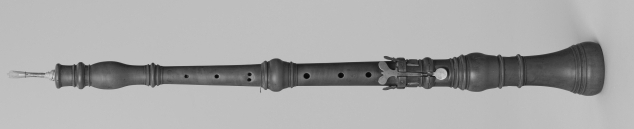
\includegraphics[width=0.9\textwidth]{F4_09somePngOboeBaroqueDennerMIR370}%.png
}
\caption{\label{fig:asIsPng}Some png-picture, directly included }
\end{figure}
